\chapter{Result and Discussion} % Main chapter title

\label{Chapter2.75} % Change X to a consecutive number; for referencing this chapter else where, use \ref{ChapterX}
%----------------------------------------------------------------------------------------
%	SECTION 1
%----------------------------------------------------------------------------------------

%-----------------------------------
%	SECTION 2
%-----------------------------------
\section{Compilation of data}
To investigate the spectral diffusion behaviour, recorded time-resolved spectra for each of the POI before and after treatment. After the first oxidation, for better characterisation, time-resolved spectra are measured not only with one but multiple excitation polarisation. This leaves large amount of spectra files (almost 32,000 spectra!), besides visualizing the movement of lines into color maps, we need better tools to evaluate the spectral stability, a way to compile dozens, sometimes even hundreds of spectra into one single value that represents the spectral stability of a POI.

Normalized cross-correlation evaluates the similarity between 2 patterns, the closer to 1, the higher the similarity. Here we compare the time-resolved PL spectra from every time tick with the first spectrum, the average value of this series of normalized cross-correlation reflects the general level of spectral stability of the measured point.


\section{Nanodiamond size and spectral stability}

The observation of nanodiamond with SEM [fig.] fits the expectation, that after the centrifuging size selection, batch1 contains smaller nanodiamonds than batch2.  
When comparing the time-resolved spectra from sample1508 and sample1510, which were taken at 4K, with an excitation power of 120$\pm$10uW, it can be observed that the spectra from sample1510 shows more spectral diffusion. The calculation of mean normalized cross-correlation confirmed the observation. As plotted in the histogram \ref{fig:histogram-of-normalized-cross-correlation12}, the distribution of mean normalized cross-correlation nanodiamond from batch1 is much closer to 1 than from nanodiamond batch2.

As discussed in Chapter 1, in nitrogen doped diamond, to match up the chemical potential inside the diamond and on the surface, a depletion layer was formed beneath the surface, where the valence band and conducting band are bended towards up. The width of the depletion layer differs by the concentration of the donor and is around 80nm in moderately doped diamond (N$_{D}$=10$^{-16}/cm^{3}$) \cite{diederich_electron_1998}

Since the donor level of nitrogen is rather deep (1.7eV) below the minimum of conduction band, it is very hard to thermally ionize the donors at low temperature, but with the excitation of 532nm(2.33eV) green laser, it is possible to excite the electrons from the donor level to the conduction band. 

So in our case, there is higher chance for nanodiamonds from batch1, which are of smaller sizes, to obtain SiV$^{-}$s sitting inside the bended band than those ones of larger diameters, like the ones from batch2. For more information I looked up the position of SiV$^{-}$s in the paper \cite{rogers_multiple_2013}, where SiV$^{-}$s in bulk diamond are reported to have very good long term spectral stability (no spectral position variation in 90min), interestingly, the distance of SiV$^{-}$s from the surface is larger than 2um, which means they sat in the bulk diamond region instead of band bended region. 


\section{Excitation power and spectral stability}

Sample 1508 was excited with decreasing excitation power. The left column of \ref{fig:powerdependenceref11} shows the changes of time-resolved spectra of POI ref11, the most obviously diffusing line is the one between 738nm and 739nm, whose spectral position changed almost 1nm in 300s. As the excitation power decreases, the diffusion become less intense.

The result of cross correlation is can be seen in \ref{fig:powerdependencybeforeafteroxidation}, where each dot represents a POI in the sample. As shown in the figure, the general level of spectral diffusion decreases as the excitation power decreases. 

A possible reason for this behaviour is the optical transition between the Nitrogen donor level and the conduction band has been involved in the excitation of SiV$^{-}$. The nitrogen donor level lies 1.7eV below the minimum of diamond conduction band \cite{diederich_electron_1998}, the spontaneous emission between the valence band and the donor level is capable of excite the SiV$^{-}$ from ground state to the first excited state.

 
\begin{figure}[h]
\centering
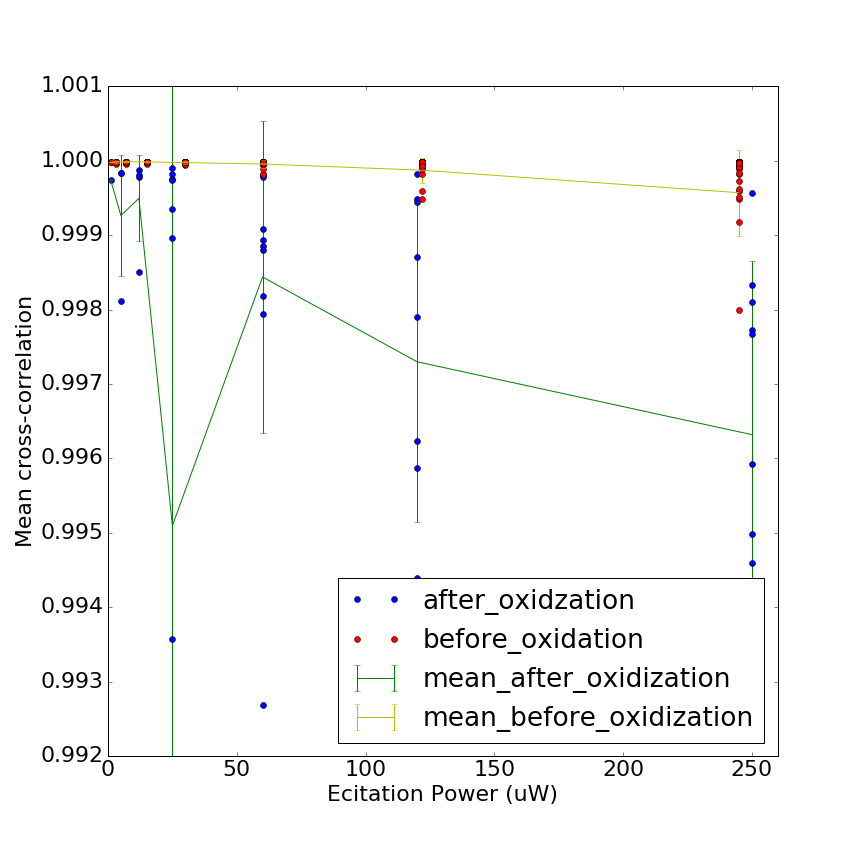
\includegraphics[width=0.7\linewidth]{Figures/pic/powerdependencybeforeafteroxidation}
\caption{Powerdependency of nanodiamond batch2, before and after first oxidation.}
\label{fig:powerdependencybeforeafteroxidation}
\end{figure}

\section{Temperature and spectral stability}
Comparing the mean normalized cross-correlation of sample 1510 from 4.7K and 20K in \ref{fig:histogram-of-normalized-cross-correlation12}, no significant difference between the two temperatures has been found,which fits the expectation. Since the assumption is that, the donors are ionized with the help of laser, the band bending should stay the same as long as the excitation power is not changed, so shall the spectral diffusion.
I consider this result not solid enough as only 3 points were measured for the 4.7K measurement. But it would be interesting to collect more data to justify the prediction.

\section{Excitation polarisation and spectral stability}

\begin{figure}[h]
\centering
\includegraphics[width=0.7\linewidth]{"Figures/pic/excitation polarisation"}
\caption{Mean normalized cross-correlation against excitation polarisation. The error bar stand for standard deviation}
\label{fig:excitation-polarisation of untreated nanodiamond batch 2}
\end{figure}

The polarisation of photoluminescence has been measured in \cite{rogers_all-optical_2014}, where the excitation polarisation patterns suggested that the SiV$^{-}$ is aligned along the <111> axis of diamond crystal. A set of dots of none-polarisation dependency(excite from the z axis of the SiV$^{-}$), or symmetric patterns that are rotationally separate from each other by an angle of 60$^{o}$ with population contrast of 60$\%$ are expected to be observed when excite the SiV$^{-}$ along crystal axis <111>. The polarisation pattern generated from other orientations can be considered as shadowing the <111> axis from respective angle.

In the measurement of excitation polarisation on sample 1510, time-resolved PL spectra are taken with different excitation polarisations. We do noticed some POIs behaved differently when excited with different beam polarisation\ref{fig:polarisationref03}. But no clear polarisation pattern has been acquired. Further cross-correlation calculation \ref{fig:excitation-polarisation of untreated nanodiamond batch 2} showed polarisation dependency like pattern in poi ref12, while the other two pois have no clear pattern.

Further excitation polarisation-resolved spectra were taken on the same sample. In some of the spectra, polarisation-related periodic pattern can be seen on some of the lines, while the sum up pattern give no polarisation dependency.


\begin{figure}[h]
\centering
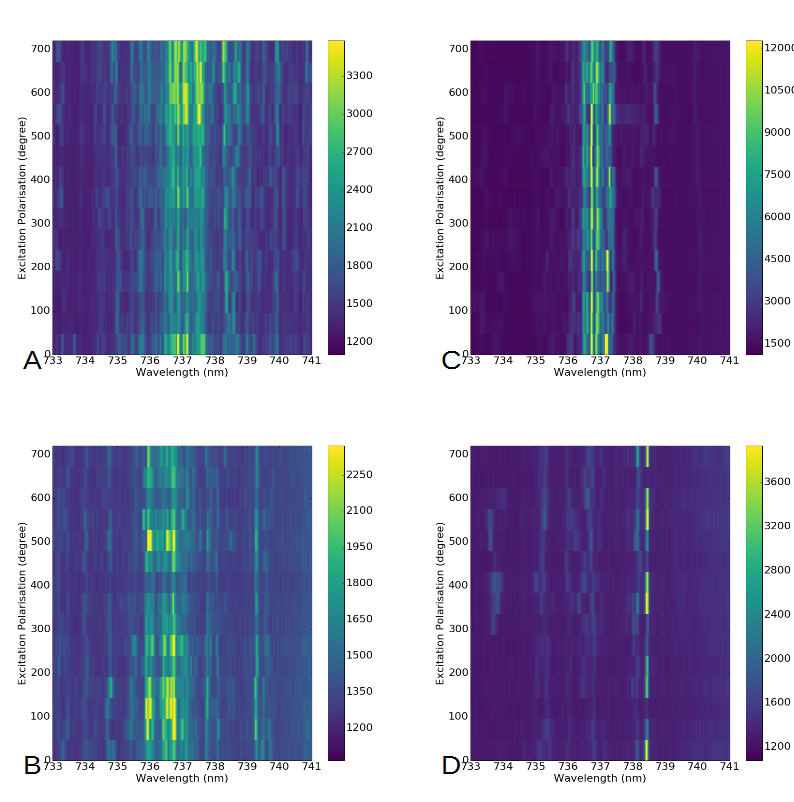
\includegraphics[width=1\linewidth]{Figures/pic/polarisationexcitation}
\caption{4 Excitation polarisation-resolved spectra from sample 1510, A: ref16, B:ref13, C:ref15, D:ref12. Some of the lines in these spectra show polarisation dependency, most significantly can be seen in ref12 }
\label{fig:polarisationexcitation}
\end{figure}
 
\begin{figure}[h]
\centering
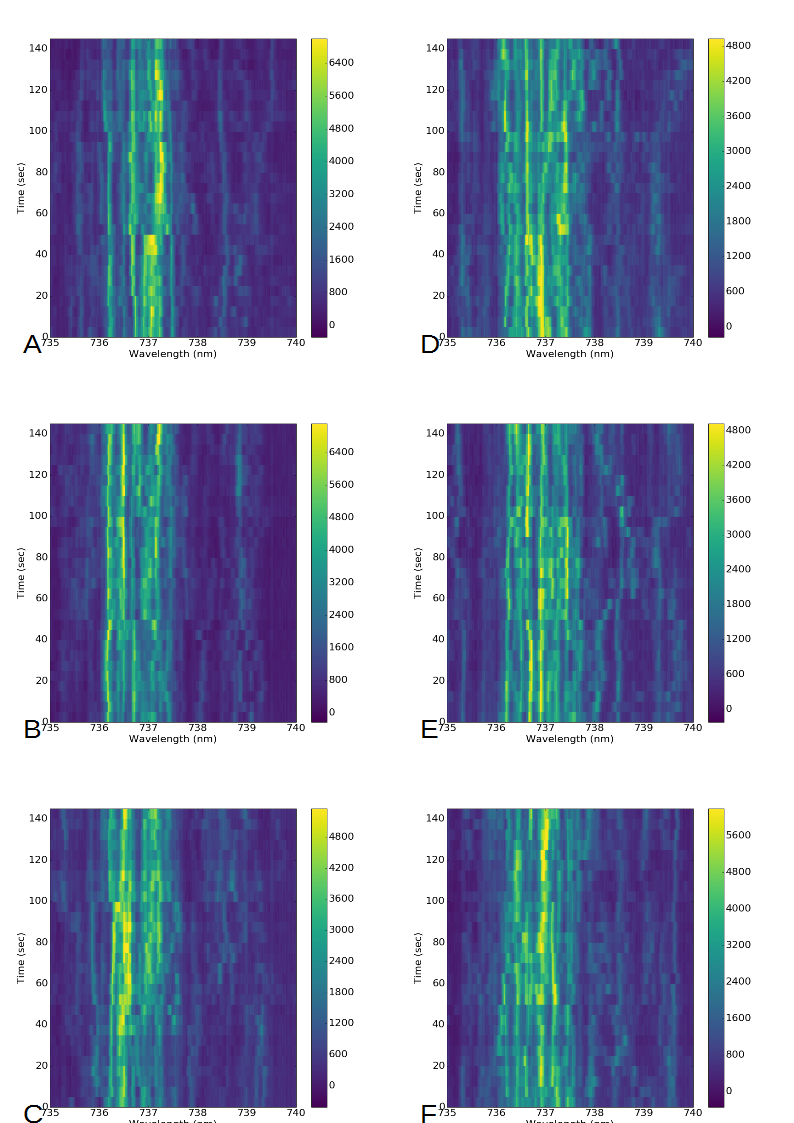
\includegraphics[width=1\linewidth]{Figures/pic/polarisationref03}
\caption{Time-resolved spectra of poi ref03, sample1510 with different excitation polarisation. Polarisation of the excitation beam: A: 0$^{o}$, B: 40$^{o}$, C: 80$^{o}$, D: 120$^{o}$, E: 160$^{o}$, F: 200$^{o}$. This figure continues in \ref{fig:polarisationref032} }
\label{fig:polarisationref03}
\end{figure}
\begin{figure}[h]
\centering
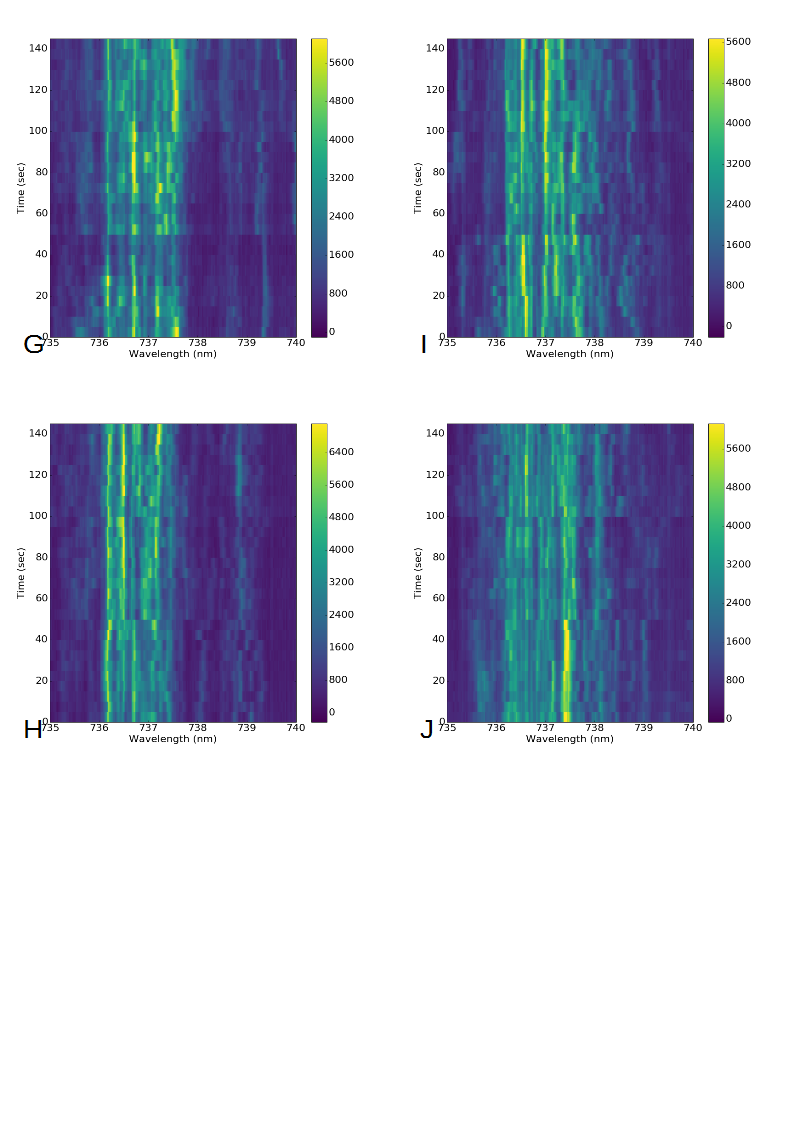
\includegraphics[width=1\linewidth]{Figures/pic/polarisationref03_2}
\caption{This figure follows \ref{fig:polarisationref03}. Excitation Polarisation: G: 240$^{o}$, H: 280$^{o}$, I: 320$^{o}$, J: 360$^{o}$ }
\label{fig:polarisationref032}
\end{figure}


\begin{figure}[h]
\centering
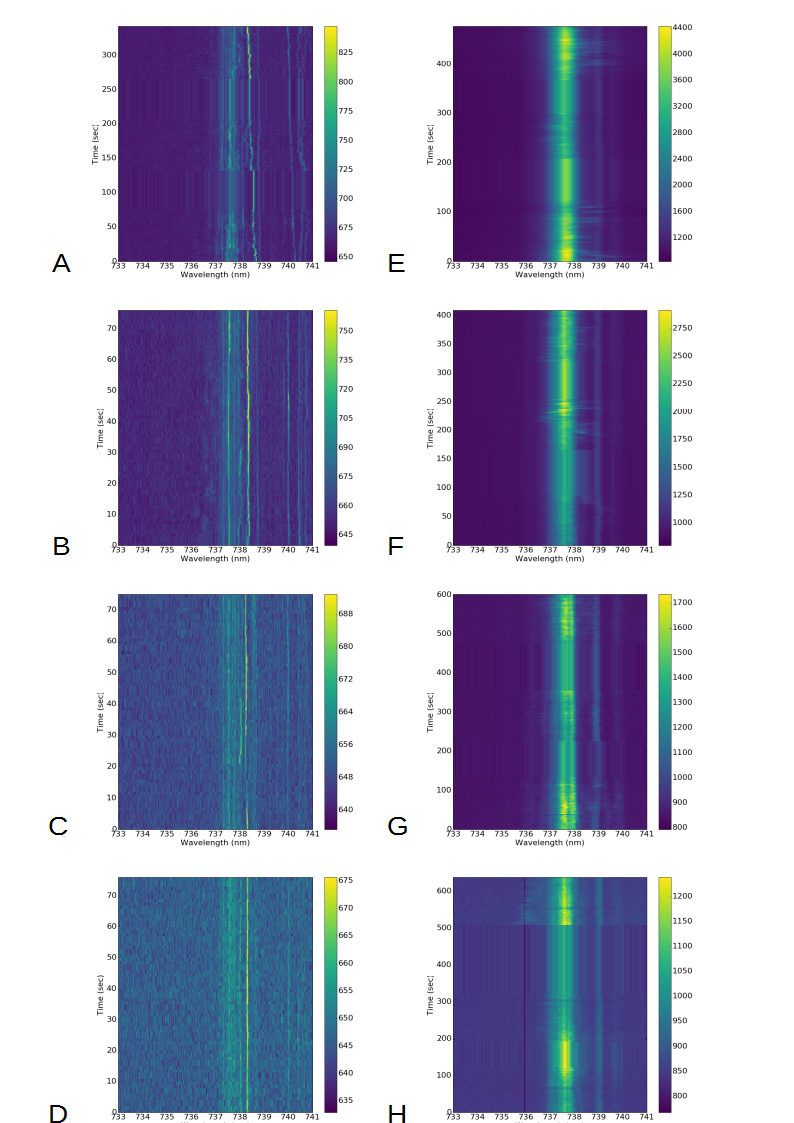
\includegraphics[width=1\linewidth]{Figures/pic/powerdependenceref11}
\caption{Left column: time resoved PL spectra of point ref11, sample1508 before the first aerobic oxdiation with different excitation power (A:250uW, B:122uW, C:60uW, D:30uW). Right column:time resoved PL spectra of point ref11, sample1508 after the first aerobic oxdiation with different excitation power (A:250uW, B:120uW, C:60uW, D:25uW). The spectra were ploted in the order of real time, the stretched pixel is the blank for refocus.}
\label{fig:powerdependenceref11}
\end{figure}
\begin{figure}[h]
\centering
\includegraphics[width=0.7\linewidth]{"Figures/pic/Histogram of normalized cross-correlation_1_2"}
\caption{Histogram comparing the normalized mean value of cross-correlation between untreated sample 1508 (nanodiamond batch2) at 4.7K and sample 1510(nanodiamond batch1) at 4.7K and 20K. The height of the bars are normalized by the integration over bins. The time resolved spectra of sample 1510 was recorded with 2 different excitation polarisation, they are separated with solid and dashed lines.}
\label{fig:histogram-of-normalized-cross-correlation12}
\end{figure}
\begin{figure}[h]
\centering
\includegraphics[width=0.7\linewidth]{"Figures/pic/Histogram of normalized cross-correlation_1_H"}
\caption{Histogram comparing the normalized mean value of cross-correlation between untreated sample 1510 and hydrogen plasma treated sample 1512 (both spin coated with nanodiamond from the batch1).The height of the bars are normalized by the integration over bins.  }
\label{fig:histogram-of-normalized-cross-correlation1h}
\end{figure}
\begin{figure}[h]
\centering
\includegraphics[width=0.7\linewidth]{"Figures/pic/Histogram of normalized cross-correlation_1_H_2"}
\caption{Histogram comparing the normalized mean value of cross-correlation between untreated sample 1508(nanodiamond batch2) and hydrogen plasma treated sample 1512(nanodiamond batch1).The height of the bars are normalized by the integration over bins.  }
\label{fig:histogram-of-normalized-cross-correlation1h2}
\end{figure}

\begin{figure}[h]
\centering
\includegraphics[width=0.7\linewidth]{"Figures/pic/Histogram of normalized cross-correlation_2_o"}
\caption{Histogram comparing the normalized mean value of cross-correlation between untreated and oxidized sample 1509(nanodiamond batch1) at 4.7K. The height of the bars are normalized by the integration over bins. }
\label{fig:histogram-of-normalized-cross-correlation2o}
\end{figure}


\section{Aerobic Oxidation and Spectral stability}

\paragraph{}The initial target for aerobic oxidation is to selectively remove graphitic defects(the first oxidation) and to generate bulk diamond-like surfaces(the second oxidation). The second oxidation, which was operated on sample 1510, didn't turn out as we wishes, offering no useful data on SiV$^{-}$. The first oxidation on sample1508 and 1509 introduced dark spots that are visible in optical microscopy images, and very bright spots containing no SiV$^{-}$ signal in confocal measurements. These are suspected to be exotic, as the furnace has been used for other materials. Yet it was managed to re-find some of the pois from sample1508.

The aerobic oxidation has greatly enhanced the photoluminescence of the sample in general, including SiV$^{-}$ and background. The left column of \ref{fig:prepostoxidationspectra} shows the comparison of spectrometer recorded intensity between before and after oxidation, as can be seen in ref3 and other points, the magnification of the enhancement is not uniform. The broadening of peak is also observed. The number of peaks that are distinguishable has decreased after the oxidation. While the spectra before oxidation consists of multiple thinner peaks, the spectra after oxidation contains broader peaks joining with each other. It is suspected that the spectrometer was not well aligned, which results in the broadening of peak  and the disappearance of fine structure. Despite the broadening, an visible enhancement \ref{fig:prepostoxidationtimeresolvespectra} in the spectral diffusion was also noticed, mean cross-correlation comparison can be found in \ref{fig:histogram-of-normalized-cross-correlation2o}. The power dependency of spectral diffusion (mean cross-correlation) is plotted in \ref{fig:powerdependencybeforeafteroxidation}, with similar trend as before oxidation: the spectral diffusion increases as excitation power increases. The drop of 30uW is due to an extreme point which obtained very noisy background, that is related to the suspected exotic luminescence from the oxidation process. 

\begin{figure}[h]
\centering
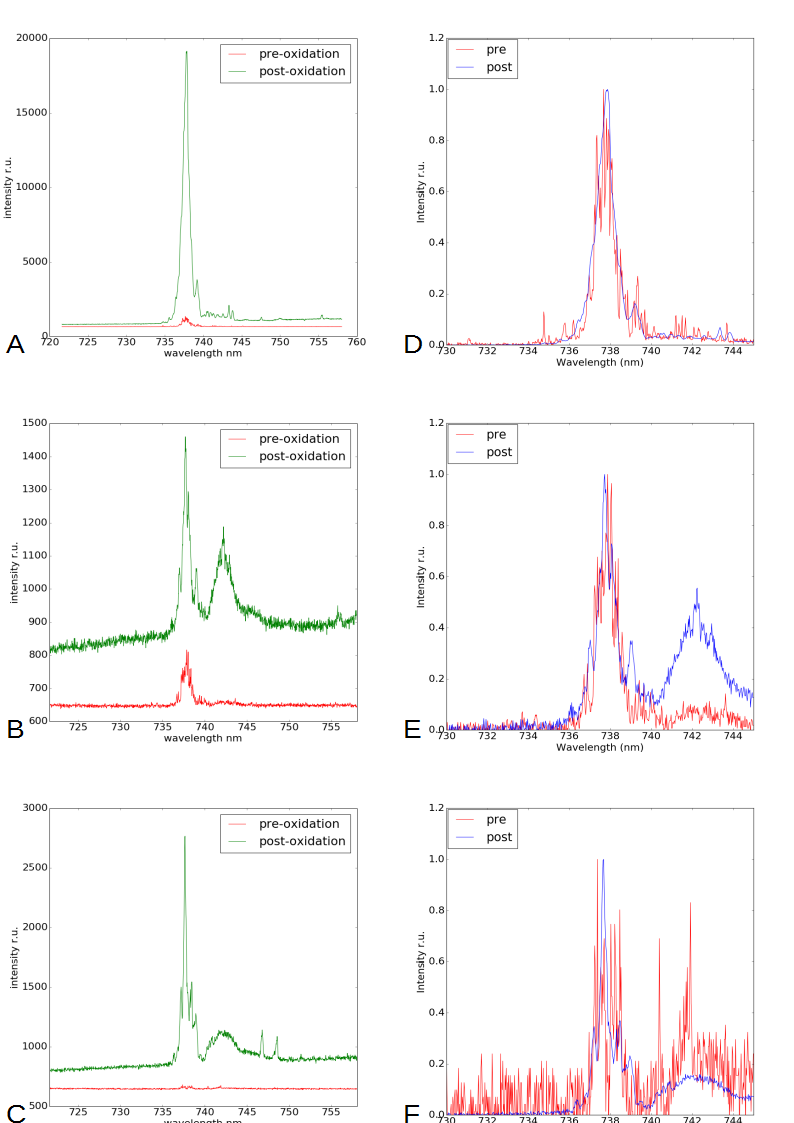
\includegraphics[width=1\linewidth]{Figures/pic/prepostoxidationspectra}
\caption{Comparison between the PL Spectra of 3 of the pois from sample1508. Left column: real value. Right column: normalized spectra. The spectra were recorded with 120uW of excitation power with 532nm green laser and 1s of exposure time. A,D: ref4, B,E: ref3, C,F: ref5.}
\label{fig:prepostoxidationspectra}
\end{figure}

\begin{figure}[h]
\centering
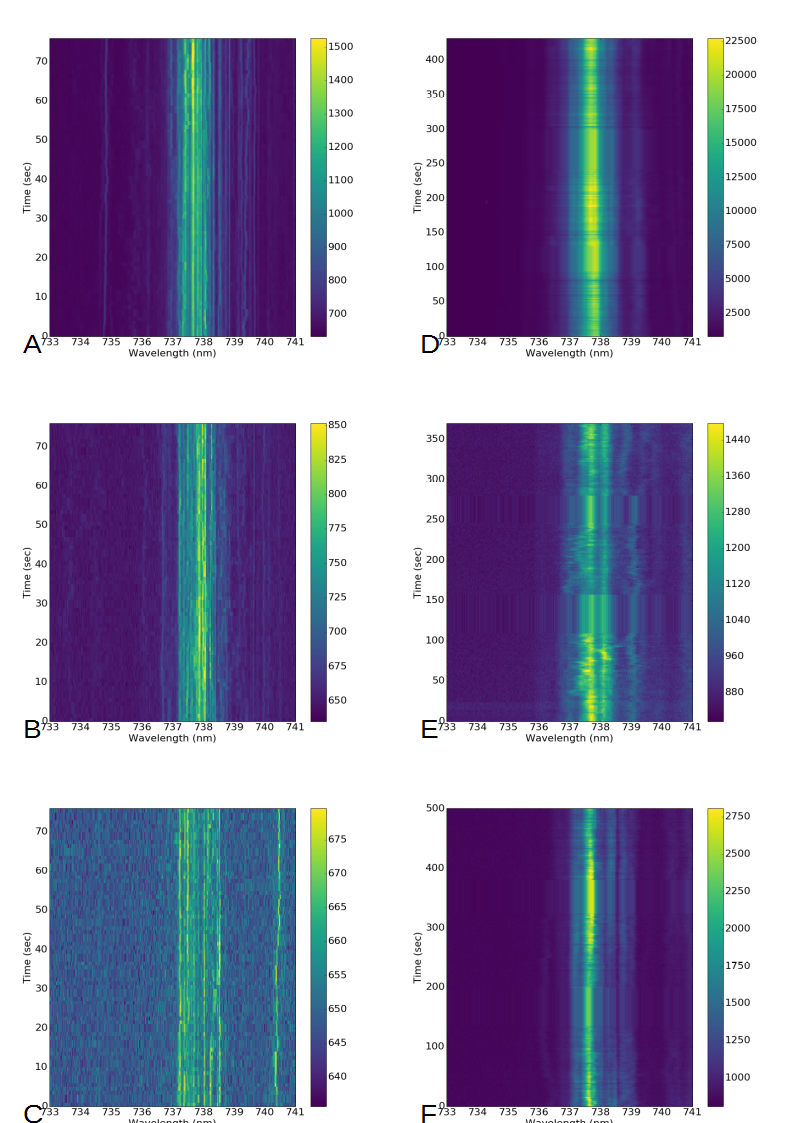
\includegraphics[width=1\linewidth]{Figures/pic/prepostoxidationtimeresolvespectra}
\caption{The time-resolved spectra of pois from \ref{fig:prepostoxidationspectra}. The spectra were also recorded with 120uW of excitation power with 532nm green laser and 1s of exposure time. Left column: before oxidation, right column: after oxidation. A,D: ref4, B,E: ref3, C,F: ref5.The spectra were ploted in the order of real time, the stretched pixel is the blank for refocus.}
\label{fig:prepostoxidationtimeresolvespectra}
\end{figure}


\section{Hydrogen termination and Spectral stability}

Hydrogen terminated diamond surface posses negative electron affinity \citep{maier_electron_2001,ristein_electronic_2000,diederich_electron_1998} and is related to the depletion of NV centres in diamond \citep{stacey_depletion_2012}. After hydrogen plasma treatment on sample1512(nanodiamonds batch1) as mentioned in \ref{Chaper2.5}, time-resolved PL and excitation polarisation-resolved PL were recorded at 20K.

The time resolved pattern has been plotted out in \ref{fig:hydrogenterminationtimeresolve}, a visibly improvement in the spectral stability is shown. The comparison of mean cross-correlation of untreated nanodiamonds batch1 and hydrogenated ones can be found in \ref{fig:histogram-of-normalized-cross-correlation1h}, which agrees with the observation. As reference the comparison between nanodiamonds batch2 and hydrogen terminated batch1 was also plotted \ref{fig:histogram-of-normalized-cross-correlation1h2}. The hydrogenated nanodiamonds also responds the changes in excitation polarisation better. Clear polarisation dependency pattern can be seen in \ref{fig:hydrogenterminationpolarisation}. It has been noticed in the polarisation pattern of untreated nanodiamonds, that despite the general pattern reflects no polarisation dependency, some of the lines can still be seen changing periodically with the excitation polarisation. If we look closely at figure B and E in \ref{fig:hydrogenterminationpolarisation}, between 735nm and 737nm, there is a broader and less bright band whose not only intensity but also width changes with excitation polarisation. This pattern has also been seen in the pre-treatment sample.

 

\begin{figure}[h]
\centering
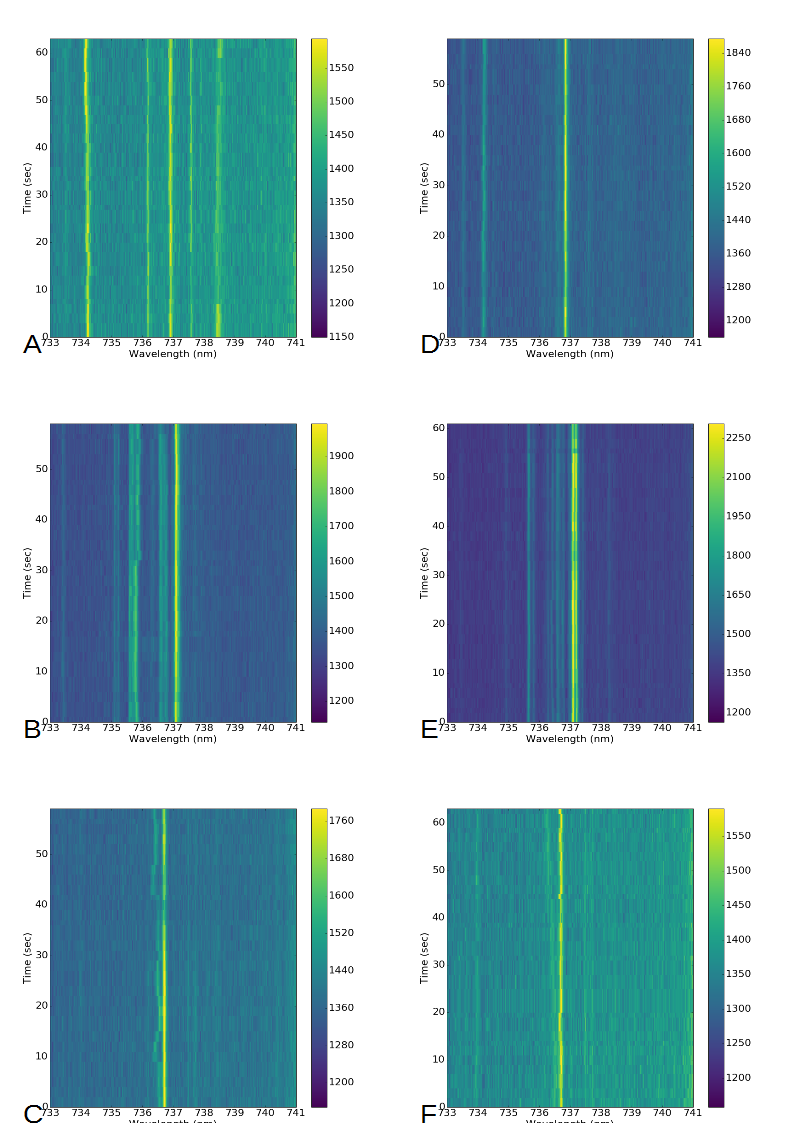
\includegraphics[width=1\linewidth]{Figures/pic/hydrogenterminationtimeresolve}
\caption{Time-resolved PL spectra of poi ref18, ref19 and ref20 from sample1512 at 20K. The excitation polarisation of left and right column are perpendicular to each other.
A,D: ref20, B,E: ref19, C,F: ref18}
\label{fig:hydrogenterminationtimeresolve}
\end{figure}

\begin{figure}[h]
\centering
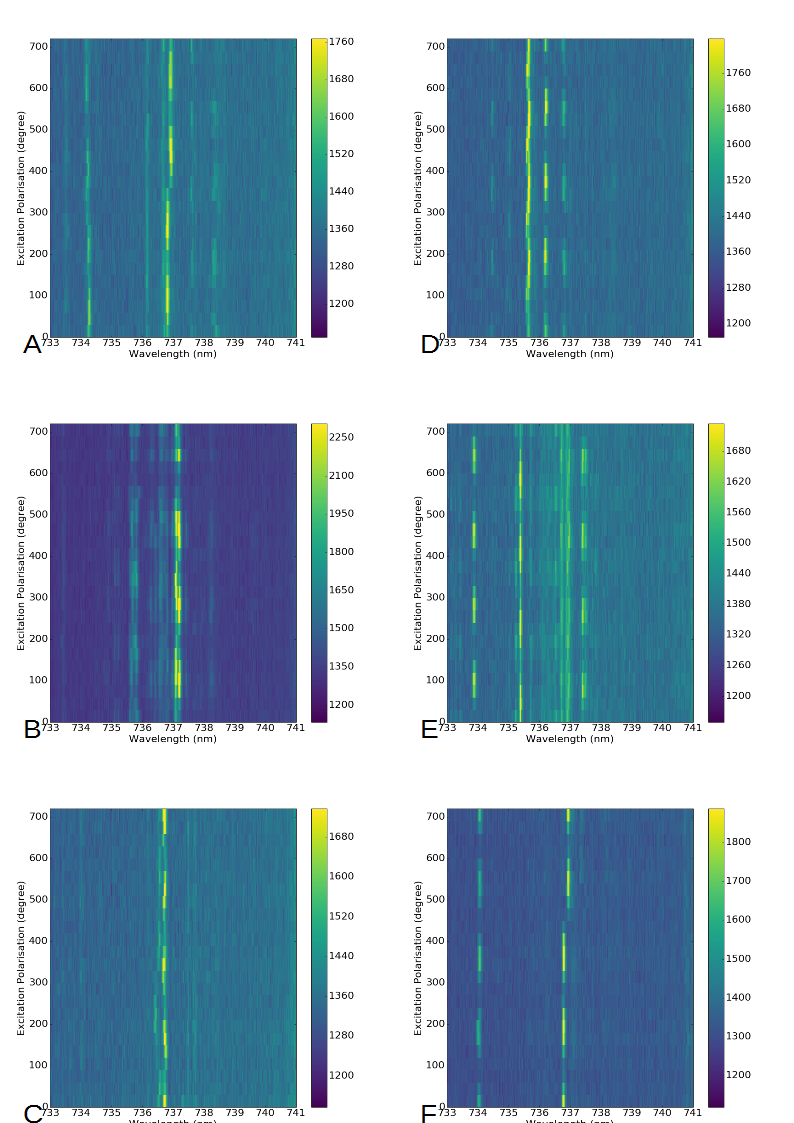
\includegraphics[width=1\linewidth]{Figures/pic/hydrogenterminationpolarisation}
\caption{The excitation polarisation-resolved spectra of pois from sample1512 at 20K. A: ref20, b:ref19, C:ref18, D:ref15, E:ref13, F:ref12.}
\label{fig:hydrogenterminationpolarisation}
\end{figure}

\section{Discussion}

The size effect of colour centre in nanodiamonds is often related the the surface band bending phenomena. Here I try to explain the phenomena that has been observed with very wild guess and hypothesis.

As the samples are nitrogen doped, it is expected to have a upward band-bending, with a fermi level between the conduction band and the donor level. When the surface chemical potential is low enough, it is possible to have the donor level, even valence band maximum of the bulk region crossing the fermi level near the surface, which results in the accumulation of holes. 

The Nitrogen atom level lies 1.7eV below the minimum of the conduction band \citep{diederich_electron_1998}, at cryogenic temperature, the main electron source is the photon-excited electrons, with our 532nm excitation laser, it is not possible to excite electron from the valence band, but possible from the donor level.

\begin{figure}[h]
\centering
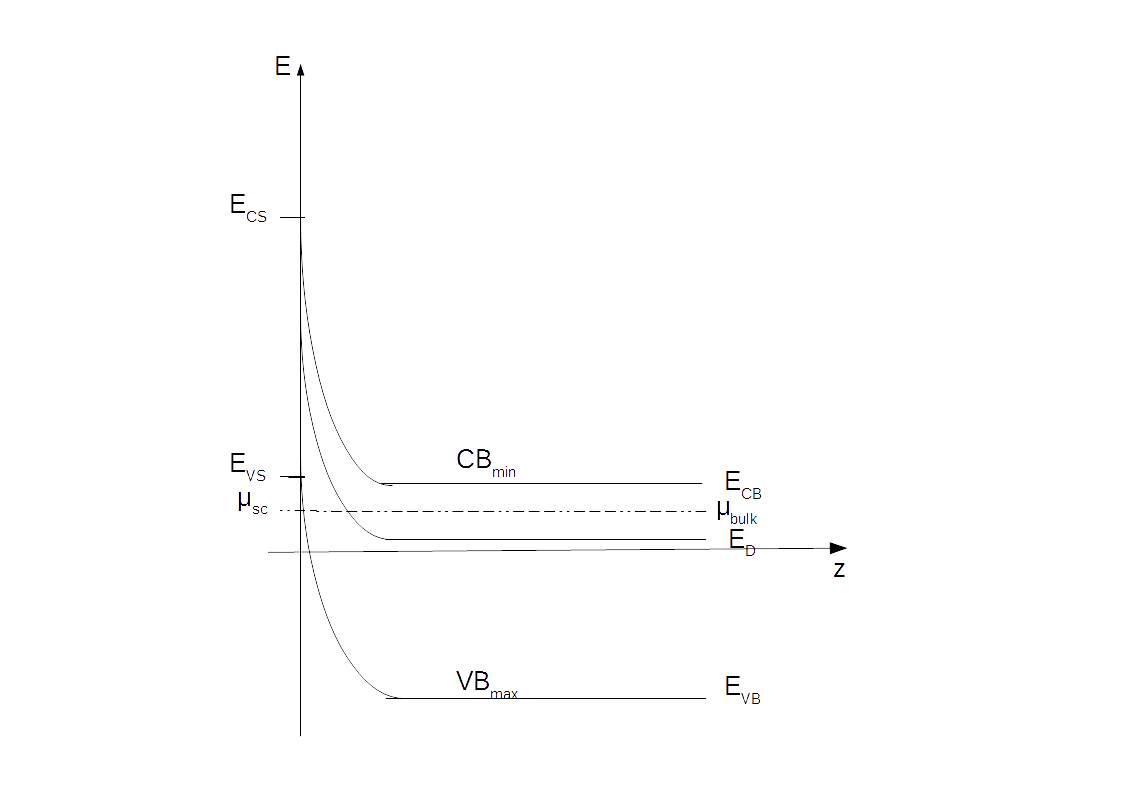
\includegraphics[width=1\linewidth]{Figures/pic/nbandbend}
\caption{Sketch of band bending in n doped nitrogen vacancy. The cross over of fermi level and nitrogen atom level may cause the accumulation of holes. E$_{D}$: donor level, the nitrogen atom level. E$_{CB}$: bulk conduction band minimum. E$_{VB}$: bulk valence band maximum. E$_{CS}$: surface conduction band minimum. E$_{VS}$: surface valence band maximum. $\mu_{SC}$: surface chemical potential. $\mu_{bulk}$: bulk chemical potential.} 
\label{fig:nbandbend}
\end{figure}
 

Since the accumulation of holes at the nitrogen atom level, the electrons from the conduction band are encouraged to recombine with the holes and emit photons. Since 1.7eV is larger than the band gap between SiV$^{-}$ ground state and the first excited state, these spontaneous emission can be involved in the excitation of SiV$^{-}$s. 
While the polarisation of spontaneous emission is not relevant to the excitation polarisation, the excitation polarisation pattern of SiV$^{-}$ may not be solely the reflection of excitation polarisation but also the polarisation of spontaneous emission from the conduction band, which explains the patterns in \ref{fig:polarisationexcitation}.

As excitation power increases, more electrons are excited into the conduction band, which leads to further increase of spontaneous emission, which can be related to the power dependency of spectral diffusion in \ref{fig:powerdependencybeforeafteroxidation}, \ref{fig:powerdependenceref11}.